\chapter{Fundamentos t\'eoricos}
\label{cap:fundamentosTeoricos}

Este capítulo aborda los fundamentos teóricos necesarios para comprender las redes Peer-to-Peer (P2P), comenzando con su definición y evolución histórica.
También, se analizan los tipos de arquitecturas P2P más comunes y los distintos protocolos que permiten su funcionamiento, como TCP y UPnP.

\section{Introducción a las redes P2P}
Las redes P2P son sistemas de comunicación que se caracterizan por su arquitectura descentralizada, donde todos los nodos de la red desempeñan roles equivalentes.
Esto significa que los nodos actúan tanto como clientes, solicitando recursos, como servidores, compartiendo datos con otros nodos.
Según \cite{schollmeier2001}, una red P2P se define por su capacidad para que los nodos compartan recursos directamente entre ellos, sin depender de una entidad central que coordine o gestione las interacciones.
Este enfoque fomenta la resiliencia y la escalabilidad, ya que la red no depende de un único punto de fallo.

En contraste, el modelo cliente-servidor tradicional se basa en un servidor central que almacena los datos y responde a las solicitudes de los clientes.
Este modelo tiene algunas limitaciones importantes, como posibles cuellos de botella y la vulnerabilidad a fallos del servidor centralizado \cite{coulouris2011}.
Por el contrario, las redes P2P distribuyen la carga de trabajo entre todos los nodos, aprovechando la capacidad colectiva de la red para manejar grandes volúmenes de datos de manera eficiente.

\paragraph{Primera generación de redes P2P}

El desarrollo moderno de las redes P2P comenzó en 1999 con la aparición de Napster, una plataforma diseñada para compartir música.
Napster marcó un hito al permitir que los usuarios intercambiaran archivos directamente, popularizando el concepto de redes P2P \cite{oram2001}.
Su arquitectura introdujo el uso de servidores para indexar recursos, una tecnología que facilitaba la búsqueda y transferencia de archivos.
Sin embargo, su dependencia de un único punto de control lo convirtió en un objetivo legal vulnerable.
El cierre de Napster en 2001 marcó el final de esta primera etapa y el inicio de redes P2P más descentralizadas.

\paragraph{Segunda generación de redes P2P}

La segunda generación de redes P2P, representada por plataformas como Gnutella y eDonkey, eliminó los servidores centrales y adoptó modelos completamente distribuidos.
En Gnutella, por ejemplo, cada nodo se conectaba directamente con otros nodos vecinos, formando una red en malla.
Aunque esta descentralización mejoró la resiliencia de la red, también introdujo grandes retos técnicos.
Entre los principales desafíos se encontraban la búsqueda eficiente de recursos en una red distribuida y la gestión del tráfico generado por los distintos nodos \cite{risson2006}.

Por su parte, eDonkey introdujo mejoras en la forma de localizar archivos, empleando servidores auxiliares para agilizar las búsquedas, pero manteniendo la transferencia directa entre nodos.
Estas plataformas demostraron que las redes P2P podían escalar y manejar grandes cantidades de datos, pero también dejaron claro la necesidad de mejorar su funcionamiento.

\paragraph{BitTorrent y la fragmentación de archivos}

En 2001, BitTorrent marcó un punto de inflexión en la evolución de las redes P2P al introducir un nuevo enfoque para el intercambio de archivos.
En lugar de que un nodo descargara un archivo completo de otro, BitTorrent dividía los archivos en fragmentos más pequeños.
Esto permitía que un usuario descargara diferentes fragmentos de un archivo desde múltiples nodos simultáneamente, aumentando la eficiencia del ancho de banda disponible \cite{cohen2003}.
Además, los nodos comenzaban a compartir los fragmentos descargados con otros usuarios antes de completar la descarga, lo que aumentaba la colaboración entre los nodos.

Esta innovación convirtió a BitTorrent en una tecnología líder en el intercambio de archivos y popularizó el uso de las redes P2P entre los usuarios,
demostrando su capacidad para manejar grandes volúmenes de datos de manera eficiente.

\paragraph{Relevancia actual de las redes P2P}

En la actualidad, las redes P2P van más alla del ámbito del intercambio de archivos y se han adaptado a una amplia gama de aplicaciones.
Por ejemplo, en el streaming de contenido, tecnologías como WebRTC aprovechan la conectividad directa entre nodos para mejorar la latencia y reducir la carga en servidores centrales.
Además, plataformas basadas en blockchain, como Bitcoin, utilizan redes P2P para garantizar la descentralización no solo en la transferencia de datos, sino también en la gestión financiera.
Según \cite{nakamoto2008}, la arquitectura P2P es fundamental para el funcionamiento de Bitcoin, ya que elimina la necesidad de intermediarios y permite un sistema financiero más transparente y seguro.

\section{Arquitecturas de redes P2P}

La arquitectura de una red P2P define cómo los nodos se organizan para compartir recursos y comunicarse entre ellos.
Este aspecto estructural tiene un gran impacto en la eficiencia, escalabilidad y resiliencia de la red.
Existen tres tipos principales de arquitecturas en redes P2P: centralizadas, descentralizadas e híbridas \cite{schollmeier2001, risson2006}.

\subsection{Arquitecturas centralizadas}

Las arquitecturas centralizadas en redes P2P se caracterizan por la presencia de un servidor central que actúa como coordinador de las interacciones entre los nodos.
Este servidor tiene la responsabilidad de gestionar tareas clave como la indexación de los recursos disponibles, el descubrimiento de nodos y la resolución de las peticiones de los usuarios.
Los nodos individuales, por su parte, se conectan al servidor para registrar su disponibilidad y consultar la ubicación de los recursos que desean descargar \cite{schollmeier2001}.

\begin{figure}[h]
    \centering
    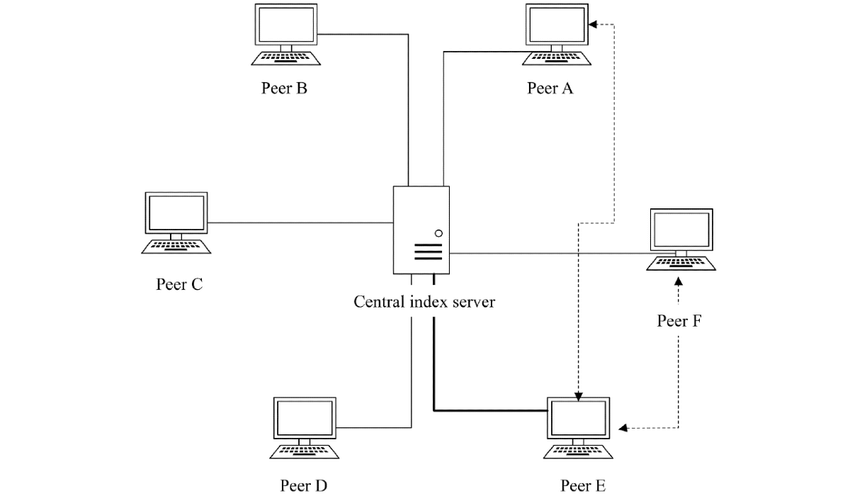
\includegraphics[width = 0.5\textwidth]{Imagenes/Vectorial/p2p_centralized}
    \caption{Ejemplo de arquitectura P2P centralizada}
    \label{fig:p2pcentralized}
\end{figure}


Un ejemplo representativo de este modelo es Napster, una de las primeras aplicaciones de intercambio de archivos en redes P2P.
En Napster, los usuarios podían buscar canciones mediante el servidor central, que les proporcionaba una lista de nodos disponibles que poseían el archivo solicitado.
Aunque las transferencias de datos se realizaban directamente entre los nodos, toda la coordinación dependía del servidor central.
Este diseño permitió a Napster ofrecer un servicio rápido y eficiente para la localización de archivos \cite{oram2001}.

Sin embargo, la dependencia de un único punto de control introdujo limitaciones significativas en las redes centralizadas.
La principal desventaja es la vulnerabilidad ante fallos del servidor, ya que su caída puede interrumpir por completo el funcionamiento de la red.
Además, esta arquitectura plantea retos relacionados con la escalabilidad.
A medida que el número de nodos y peticiones aumenta, el servidor central puede convertirse en un cuello de botella, afectando negativamente al rendimiento general del sistema.

Otro problema importante de las arquitecturas centralizadas es su exposición a riesgos legales y regulatorios.
En el caso de Napster, las demandas por infracción de derechos de autor llevaron al cierre de sus servidores en 2001, lo que dejó a los usuarios sin acceso a la red.
Este incidente manifesto la fragilidad de este modelo frente a las presiones externas, fomentando el desarrollo de alternativas más descentralizadas.

A pesar de sus limitaciones, las arquitecturas centralizadas siguen siendo útiles en ciertos escenarios donde la eficiencia y el control son prioritarios.
Por ejemplo, en redes pequeñas o sistemas donde la localización rápida de recursos es más importante que la resiliencia, un enfoque centralizado puede resultar ventajoso.
En estos casos, el servidor actúa como un mediador confiable, garantizando la consistencia y facilitando la gestión de la red.

\subsection{Arquitecturas descentralizadas}

En las redes P2P descentralizadas, todos los nodos participan con el mismo rol, asumiendo tanto funciones de cliente como de servidor.
A diferencia de las arquitecturas centralizadas, estas redes eliminan el servidor único como punto de coordinación, distribuyendo las responsabilidades entre los nodos participantes.
Este diseño aumenta significativamente la resiliencia de la red, ya que no depende de un único punto de fallo para su funcionamiento.

Una de las características distintivas de las arquitecturas descentralizadas es su capacidad para formar redes en malla.
Cada nodo establece conexiones con otros nodos vecinos, permitiendo la transferencia directa de datos sin intermediarios.
Este enfoque mejora la redundancia, ya que incluso si varios nodos fallan, la red puede seguir operando al redirigir las conexiones a través de otros caminos disponibles.
Sin embargo, esta descentralización también introduce nuevos problemas, como la necesidad de algoritmos eficientes para la localización de recursos y la gestión del tráfico de red.

Dentro de las arquitecturas descentralizadas, podemos diferenciar dos tipos principales: \textbf{estructuradas} y \textbf{no estructuradas},
cada una con características, ventajas e inconvenientes.

\subparagraph{Redes no estructuradas}

En las redes no estructuradas, los nodos se conectan de manera arbitraria, sin una organización predefinida en la topología de la red.
Estas redes se basan en conexiones dinámicas entre nodos vecinos, lo que permite la transferencia directa de datos sin intermediarios.
Este diseño mejora la redundancia, la localización de recursos es más compleja.
En estas redes, las búsquedas suelen realizarse mediante técnicas como \textit{flooding} o \textit{broadcast},
donde un nodo envía una solicitud a todos sus vecinos, y estos la retransmiten a los suyos.
Aunque estas técnicas son efectivas en redes pequeñas, generan un gran volumen de tráfico en redes más grandes, afectando significativamente el rendimiento.

La simplicidad de las redes no estructuradas las hace ideales para aplicaciones donde los recursos se distribuyen de manera uniforme y la actividad de los nodos es impredecible.
Sin embargo, no garantizan que un recurso disponible sea localizado con éxito, especialmente en redes heterogéneas y de gran escala.
Las primeras versiones de Gnutella son un ejemplo clásico de esta arquitectura, donde cada nodo actuaba de forma completamente autónoma sin una estructura definida.

\subparagraph{Redes estructuradas}

Por otro lado, las redes estructuradas imponen una organización específica sobre la topología de la red, lo que las hace más eficientes para la localización de recursos.
Estas redes utilizan algoritmos distribuidos para asignar identificadores únicos a nodos y recursos,
creando un espacio lógico donde la ubicación de cualquier recurso puede ser calculada de manera predecible.
Las tablas hash distribuidas (DHTs) son un ejemplo común de este enfoque.

En las redes estructuradas, como Chord, cada nodo y recurso se asigna a una posición dentro de un anillo lógico basado en una función hash.
Esto permite realizar búsquedas con una complejidad logarítmica, en lugar de depender de técnicas de \textit{flooding}.
Esta organización mejora la escalabilidad y la eficiencia de las redes, haciéndolas ideales para aplicaciones donde se requiere una alta predictibilidad en la localización de datos.

Aunque las redes estructuradas ofrecen claras ventajas en términos de eficiencia, también tienen algunas limitaciones.
Su implementación es más compleja y requiere que los nodos sigan estrictamente las reglas del protocolo para mantener la integridad de la red.
Además, son más vulnerables a nodos maliciosos que podrían intentar alterar la topología de la red o la asignación de recursos.

\subparagraph{Comparación y aplicaciones actuales}

Tanto las redes no estructuradas como las estructuradas tienen ventajas y desventajas que las hacen adecuadas para diferentes aplicaciones.
Las redes no estructuradas son mejores en su flexibilidad y simplicidad, lo que las hace útiles en aplicaciones donde no se requiere una localización precisa de recursos.
Por otro lado, las redes estructuradas son preferidas en sistemas donde la eficiencia y la predictibilidad son críticas,
como en aplicaciones de almacenamiento distribuido como BitTorrent.

En la actualidad, muchas arquitecturas descentralizadas han evolucionado hacia modelos híbridos, combinando elementos de ambos enfoques.
Por ejemplo, el uso de supernodos en redes no estructuradas mejora la eficiencia al centralizar parcialmente ciertas funciones,
mientras que las DHTs han sido integradas en sistemas más flexibles para manejar fallos de nodos o entornos más dinámicos.


\subsection{Arquitecturas híbridas}

Las arquitecturas híbridas combinan elementos de las arquitecturas centralizadas y descentralizadas, logrando un equilibrio entre eficiencia, escalabilidad y resiliencia.
Este enfoque es común en redes que requieren una coordinación inicial centralizada para algunas tareas, mientras mantienen la descentralización en la transferencia de datos.
Este diseño aprovecha la simplicidad de las centralizadas y la flexibilidad de las descentralizadas.

Las redes híbridas suelen tener un servidor central o un conjunto de nodos especializados que gestionan funciones como la indexación de recursos,
la localización de nodos o la autenticación de usuarios.
Sin embargo, la transferencia de datos se hace de manera descentralizada, lo que permite que la red continúe funcionando incluso si los nodos centralizados fallan.

\paragraph{BitTorrent} es el ejemplo más popular de una arquitectura híbrida que combina características de ambos tipos de redes.
En su implementación clásica, utiliza trackers, servidores centralizados que ayudan en la localización inicial de recursos.
Estos trackers proporcionan una lista de peers (nodos) que poseen partes del archivo solicitado, facilitando el inicio de las transferencias.

El diseño híbrido de BitTorrent se basa en dos componentes:
\begin{itemize}
    \item \textbf{Tracker centralizado:} Los trackers centralizados actúan como mediadores para localizar recursos.
    Aunque no participan directamente en la transferencia de datos, son esenciales para la localización de los peers.
    \item \textbf{Transferencia descentralizada:} Una vez que el tracker proporciona la información sobre los peers, la transferencia de datos se realiza directamente entre los nodos, utilizando una estructura completamente descentralizada.
\end{itemize}

La combinación de estos dos elementos permite a BitTorrent equilibrar eficiencia y escalabilidad.
Sin embargo, la dependencia de trackers introduce vulnerabilidades, como puntos únicos de fallo.
Para mitigar esto, BitTorrent ha evolucionado hacia modelos más descentralizados mediante el uso de Tablas Hash Distribuidas (DHT), que eliminan la necesidad de trackers centrales,
aumentando la robustez de la red.

\section{Protocolos de comunicación en redes P2P}

\subsection{Protocolos de transporte: TCP y UDP}
Los protocolos TCP (Transmission Control Protocol) y UDP (User Datagram Protocol) son los más usados para la comunicación de nodos en redes P2P.
Aunque ambos son esenciales para la transmisión de datos entre nodos, tienen diferencias fundamentales que los hacen más adecuados para algunos tipos aplicaciones específicas.
TCP prioriza la fiabilidad y la entrega ordenada de los datos, mientras que UDP, es más rápido y ligero, por lo que es mejor para aplicaciones que necesitan menor latencia.
En las siguientes secciones, se analizarán las características de ambos protocolos.


\subsubsection{Protocolo TCP}
El Transmission Control Protocol (TCP) es uno de los pilares fundamentales en las comunicaciones de redes Peer-to-Peer (P2P). Este protocolo de transporte confiable garantiza la entrega íntegra y ordenada de los datos entre dos nodos, lo que lo convierte en una herramienta clave para aplicaciones que priorizan la fiabilidad. TCP opera en un modelo orientado a la conexión, lo que implica que antes de transferir datos, se debe establecer una conexión entre los nodos implicados. Estas características hacen que TCP sea especialmente útil en redes P2P, incluso en entornos con condiciones de red variables.

\subsubsection*{Establecimiento de conexión: Three-Way Handshake}
El proceso de inicialización en TCP, conocido como Three-Way Handshake, permite establecer una conexión confiable entre dos nodos. Este procedimiento consta de tres pasos principales:

\begin{enumerate}
\item SYN: El nodo que inicia la conexión envía un paquete de sincronización (SYN) al nodo receptor, indicando su intención de establecer comunicación.
\item SYN-ACK: El receptor responde con un paquete de sincronización y acuse de recibo (SYN-ACK), confirmando la recepción del mensaje inicial y mostrando su disposición para continuar.
\item ACK: Finalmente, el nodo iniciador envía un paquete de acuse de recibo (ACK), completando el proceso y estableciendo la conexión.
\end{enumerate}
Este mecanismo permite a ambos nodos acordar parámetros fundamentales, como los números de secuencia iniciales y las ventanas de transmisión. Estos parámetros son esenciales para garantizar la sincronización durante la transmisión y la integridad de los datos \cite{stevens1994tcp}.

\subsubsection*{Mecanismos de fiabilidad}
TCP incluye varios mecanismos diseñados para garantizar que los datos lleguen correctamente al destino, incluso en presencia de fallos en la red:

\begin{itemize}
\item Números de secuencia: Cada byte transmitido está asociado a un número de secuencia único, que permite identificar el orden correcto de los datos y detectar duplicados.
\item Acuse de recibo (ACK): El receptor confirma la recepción de los datos enviando un mensaje ACK al emisor, indicando el próximo byte esperado. Este sistema asegura que los segmentos recibidos sean correctamente identificados.
\item Retransmisión de paquetes: Si el emisor no recibe un acuse de recibo dentro de un tiempo específico calculado dinámicamente (Retransmission Timeout, RTO), el paquete se retransmite \cite{jacobson1988congestion}.
\item Checksum: Cada segmento contiene un valor checksum que valida la integridad de los datos. Si el checksum recibido no coincide, el segmento se descarta \cite{kurose2016computer}.
\end{itemize}
Estos mecanismos garantizan la fiabilidad y precisión en la transmisión, una característica esencial para aplicaciones de intercambio de archivos en redes P2P.

\subsubsection*{Control de flujo y congestión}
Para gestionar la transferencia de datos de manera eficiente, TCP utiliza algoritmos avanzados de control de flujo y congestión:

\begin{itemize}
\item Ventana deslizante (Sliding Window Protocol): Este sistema permite al emisor transmitir múltiples segmentos sin esperar confirmación individual para cada uno, optimizando el uso del ancho de banda disponible.
\item Control de congestión: TCP adapta dinámicamente su tasa de transmisión según las condiciones de la red. Los principales algoritmos utilizados incluyen:\begin{itemize}
\item Slow Start: Inicia con un tamaño de ventana reducido, que aumenta exponencialmente hasta que se detectan signos de congestión.
\item Congestion Avoidance: Tras alcanzar la capacidad de la red, el crecimiento del tamaño de la ventana es lineal.
\item Fast Retransmit: Cuando se detectan tres ACK duplicados consecutivos, TCP asume que un paquete se perdió y lo retransmite inmediatamente, sin esperar al tiempo de retransmisión (RTO) \cite{jacobson1988congestion}.
\end{itemize}

\end{itemize}
Estos mecanismos permiten que TCP maximice el rendimiento, evitando la saturación de la red y garantizando una transferencia fluida.

\subsubsection*{Desafíos de TCP en redes P2P}
A pesar de sus ventajas, TCP enfrenta ciertos desafíos en el contexto de redes P2P:

\begin{enumerate}
\item Overhead en la gestión de conexiones: Cada conexión TCP requiere recursos significativos, como memoria y capacidad de procesamiento. En redes P2P, donde los nodos deben establecer y mantener múltiples conexiones simultáneamente, este overhead puede limitar el rendimiento \cite{cohen2003}.
\item Latencia: Los mecanismos de retransmisión y control de flujo pueden introducir retrasos, especialmente en redes congestionadas o de alta latencia.
\item Escalabilidad: La necesidad de gestionar múltiples conexiones persistentes puede convertirse en un cuello de botella en sistemas con miles de nodos.
\end{enumerate}
\subsubsection*{Relevancia de TCP en redes P2P}
A pesar de estos desafíos, TCP sigue siendo el protocolo dominante para aplicaciones P2P que priorizan la fiabilidad y la integridad de los datos. Sistemas como BitTorrent utilizan TCP para transferir fragmentos de archivos entre nodos, asegurando que cada parte se reciba de manera correcta antes de ensamblar el archivo completo. Su capacidad para operar en redes heterogéneas y manejar errores lo convierte en una herramienta esencial en el diseño de redes P2P modernas \cite{cohen2003}.


\subsubsection{Protocolo UDP}

\subsection{Configuración y gestión de conectividad en redes P2P}
\subsubsection{Problemas de NAT y firewalls}
\subsubsection{Configuración automática mediante UPnP}
\subsubsection{STUN y TURN como soluciones para NAT traversal}
